\documentclass{article}
 
\usepackage{amsmath}
\usepackage{amssymb}
\usepackage{graphicx}
\usepackage{verbatim}
\usepackage{enumerate}

\newcommand{\beq}{\begin{equation}}
\newcommand{\eeq}{\end{equation}}
%\verbatiminput{verb.txt}
\begin{document}
\title{Project 3. FYS3150}
\author{Shafa Aria}
\maketitle
\newpage
\section{Introduction}
In this project we are going to model the solar system consisting of the Sun, Earth and Jupiter with the option of adding other planets and objects as well. For starting we only focus on a Sun-Earth system and then add on planets from there on. Albeit I have decided to implement it in such a way that one can chose how many celestial objects one wishes to deal with in the program. The only equation we are really dealing with here is Newton's universal gravitational force:
$$F_G = \frac{GM_{Sun}M_{Earth}}{r^2}$$ decomposing it into the $x$ and $y$ direction, giving us:
\begin{center}
$F_{G,x} = F_G\frac{x}{r}$ \hspace{5cm} $F_{G,y} = F_G\frac{y}{r}$
\end{center}
Aside from these equations we will also be needing Newton's second law:
\begin{align*}
F = ma\\
a = \frac{F}{m}\\
\end{align*}
\begin{center}
$\frac{\mathbf{d}^2x}{\mathbf{d}t^2} = \frac{F_{G,x}}{m} \hspace{5cm} \frac{\mathbf{d}^2y}{\mathbf{d}t^2} = \frac{F_{G,y}}{m}$\\
We can again rewrite these two equations as two first order differential equations:\\
$\frac{\mathbf{d}x}{\mathbf{d}t} = v_x \hspace{5cm}  \frac{\mathbf{d}y}{\mathbf{d}t} = v_y$\\
\vspace{0.5cm}
$\frac{\mathbf{d}v}{\mathbf{d}t} = \frac{F_{G,x}}{m} \hspace{5cm}  \frac{\mathbf{d}v}{\mathbf{d}t} = \frac{F_{G,y}}{m}$
\end{center}
Equipped with the equations we are now ready to solve for our system consisting of the planets and the Sun and Pluto.

\section{Implementation}
To start off we see that we need to solve the four first order differential equations, with our method of choice being the Runga Kutta 4 method (RK4 hereafter). The RK4 algorithm is relatively straightforward: 
\begin{align*}
k_1 &= gf(t_i,x_i)\\
k_2 &= hf(t_i + h/2,y_i + k_1/2)\\
k_3 &= hf(t_i + h/2, y_i + k_2/2)\\
k_4 &= hf(t_i + h, y_i + k_3)\\
y_{i+1} &= y_i + \frac{1}{6}(k_1+2(k_2 + k_3) + k_4)
\end{align*}
For the coding, I have decided to make a simple class for the solar system which contains the mass, distance to the sun and initial positions and velocities of the planets and Pluto. Now the distances and masses would pose a problem during our calculation since we are dealing with physical quantities like $G = 6.67E-11m^3/kgs^2$ which would result in round off and arithmetic errors. For this reason we scale the planets masses to the Sun's (which is set to one) and use astronomical unit for the distance and year for the time instead of seconds. For further insight I refer to the references.

\section{Results}
Implementing the algorithm and plotting the first pair, Sun and Earth, we get the following:\\
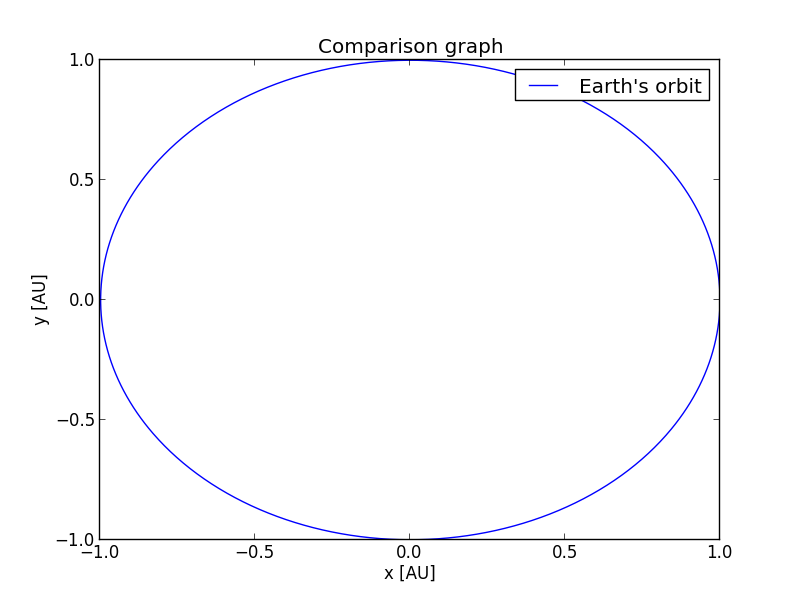
\includegraphics[scale=0.5]{figure_1.png}\\
At first I chose the initial velocity for the sun as $2\pi$ which gave a circular looking orbit. Next to find out what velocity was needed for it to escape I ran through some trial and error to find an answer starting with $v_0 = 7$AU/yr and increasing steadily: \texttt{[7, 7.4, 7,6, 8, 8.5, 9, 8.8, 8,89]}. The borderline between escape velocity and trap velocity was around $8.89$AU/yr and $9$AU/yr. After that we could see from the plot that it would just go along a straight line hence indicating escaping the gravitational field of the Sun. $8.89$AU/yr is around $42$km/s and on NASA's fact sheet, the earth's escape velocity is stated as being around $11$km/s so I assume there has been some miscalculations on my side.\\
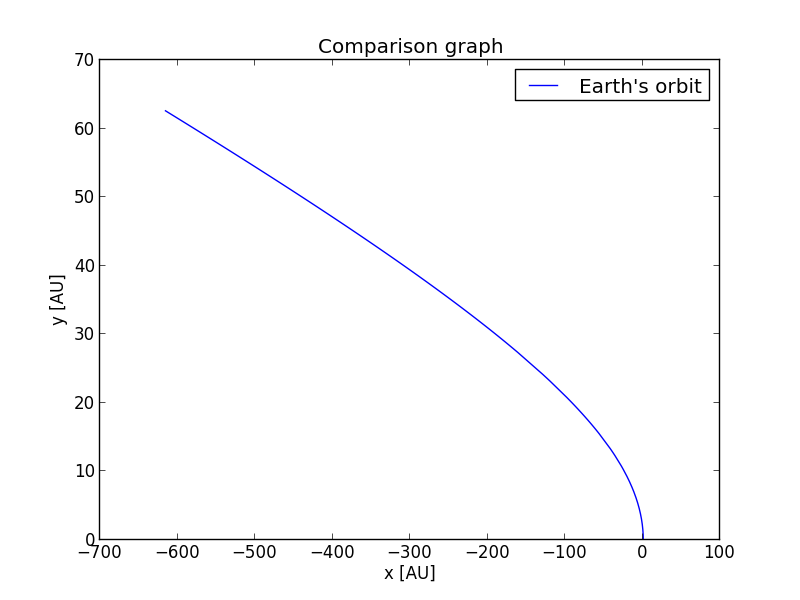
\includegraphics[scale=0.5]{figure_2.png}\\
The exact answer to the escape velocity can be found using the equation we have in our hand namely:
$$v^2r = GM_{\odot}$$
$$v_e = \sqrt{\frac{GM_\odot}{r}}$$
Now the escape velocity is just a consequence of the conservation of energy, which is in this case that the planet, with a given total energy, cannot reach states or places that have a higher potential energy than its total energy cannot be reached. In other words it can only reach places with the combination of the position and velocity which add up to the total energy with respect to the conservative gravitational force.

Going further we can now add Jupiter to our list and we get the following:\\
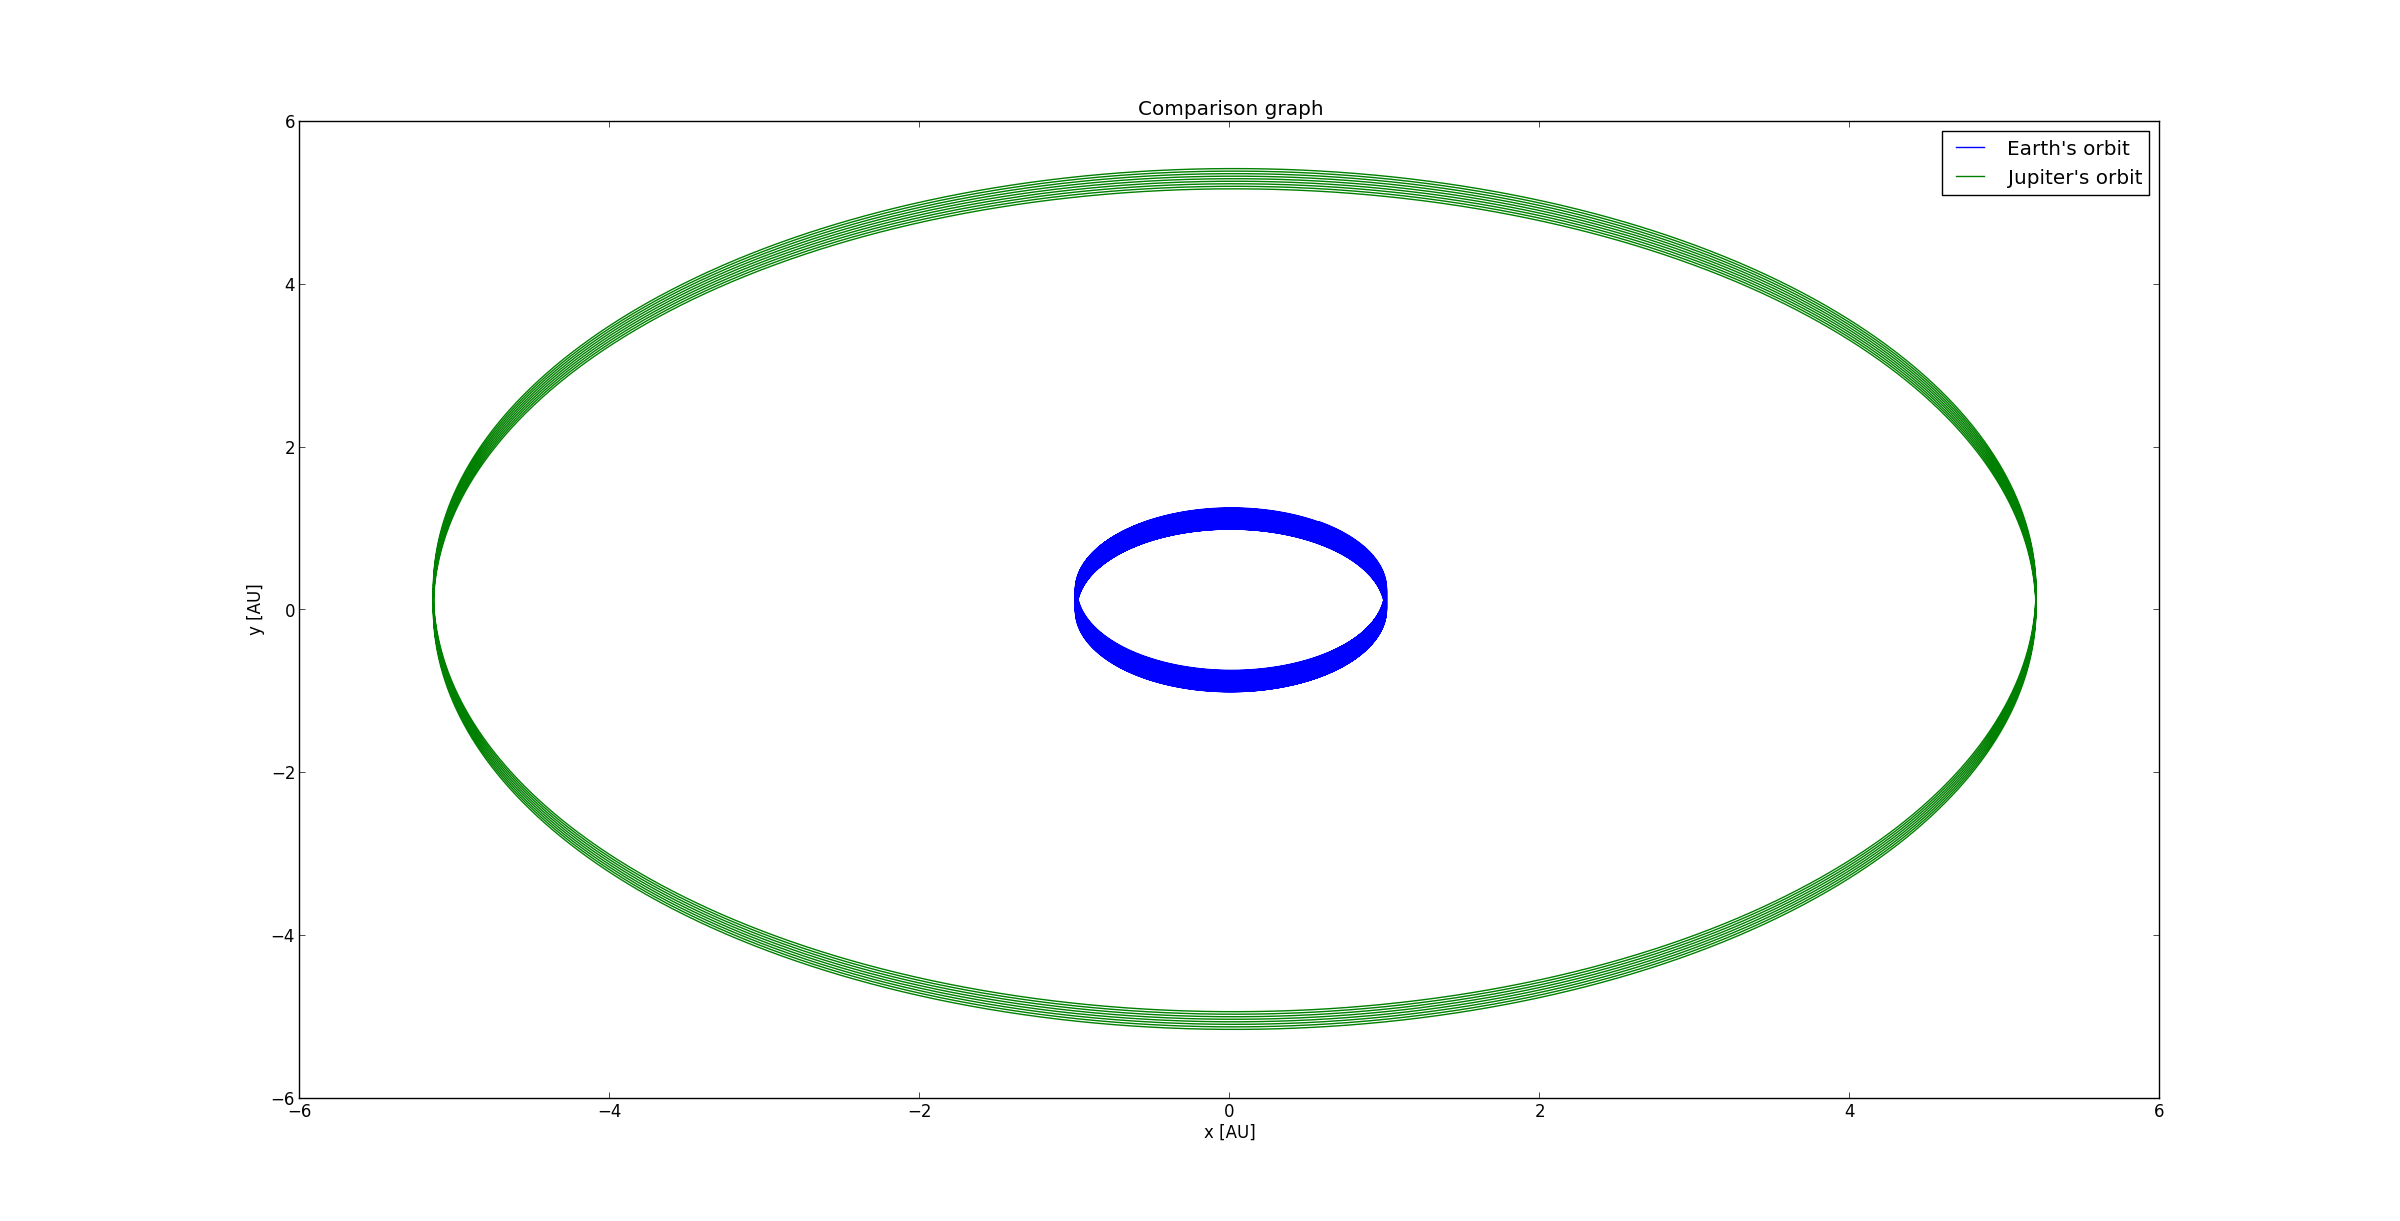
\includegraphics[scale=0.3]{figure_3.png}\\
Now we shall increase the mass of Jupiter by a factor of $10$ and $1000$. The results:\\
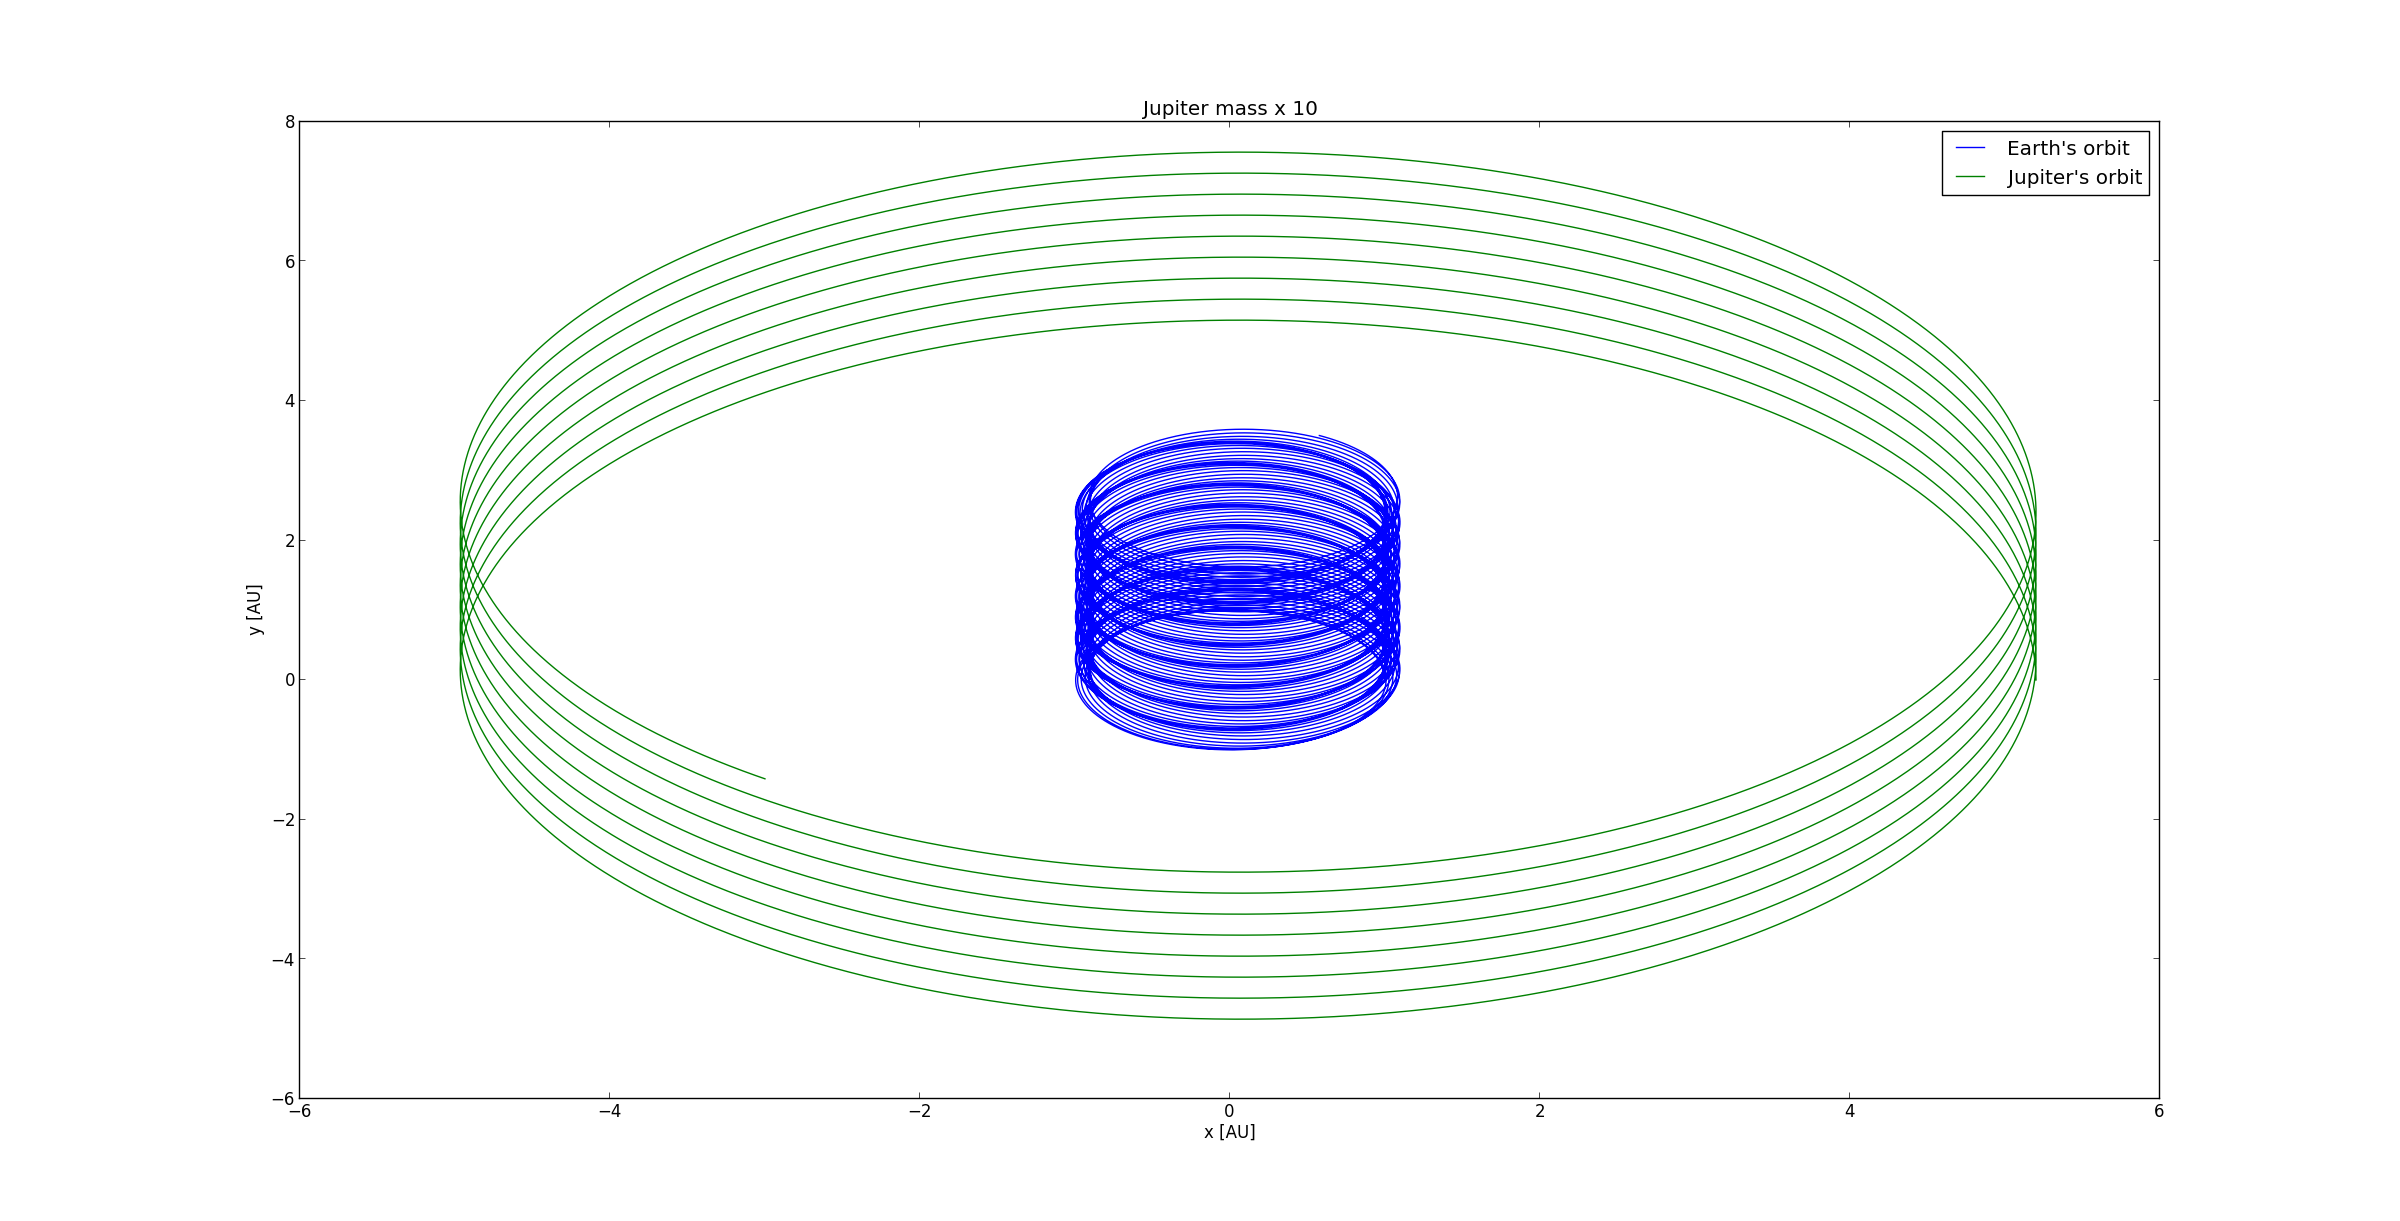
\includegraphics[scale=0.3]{figure_4.png}\\
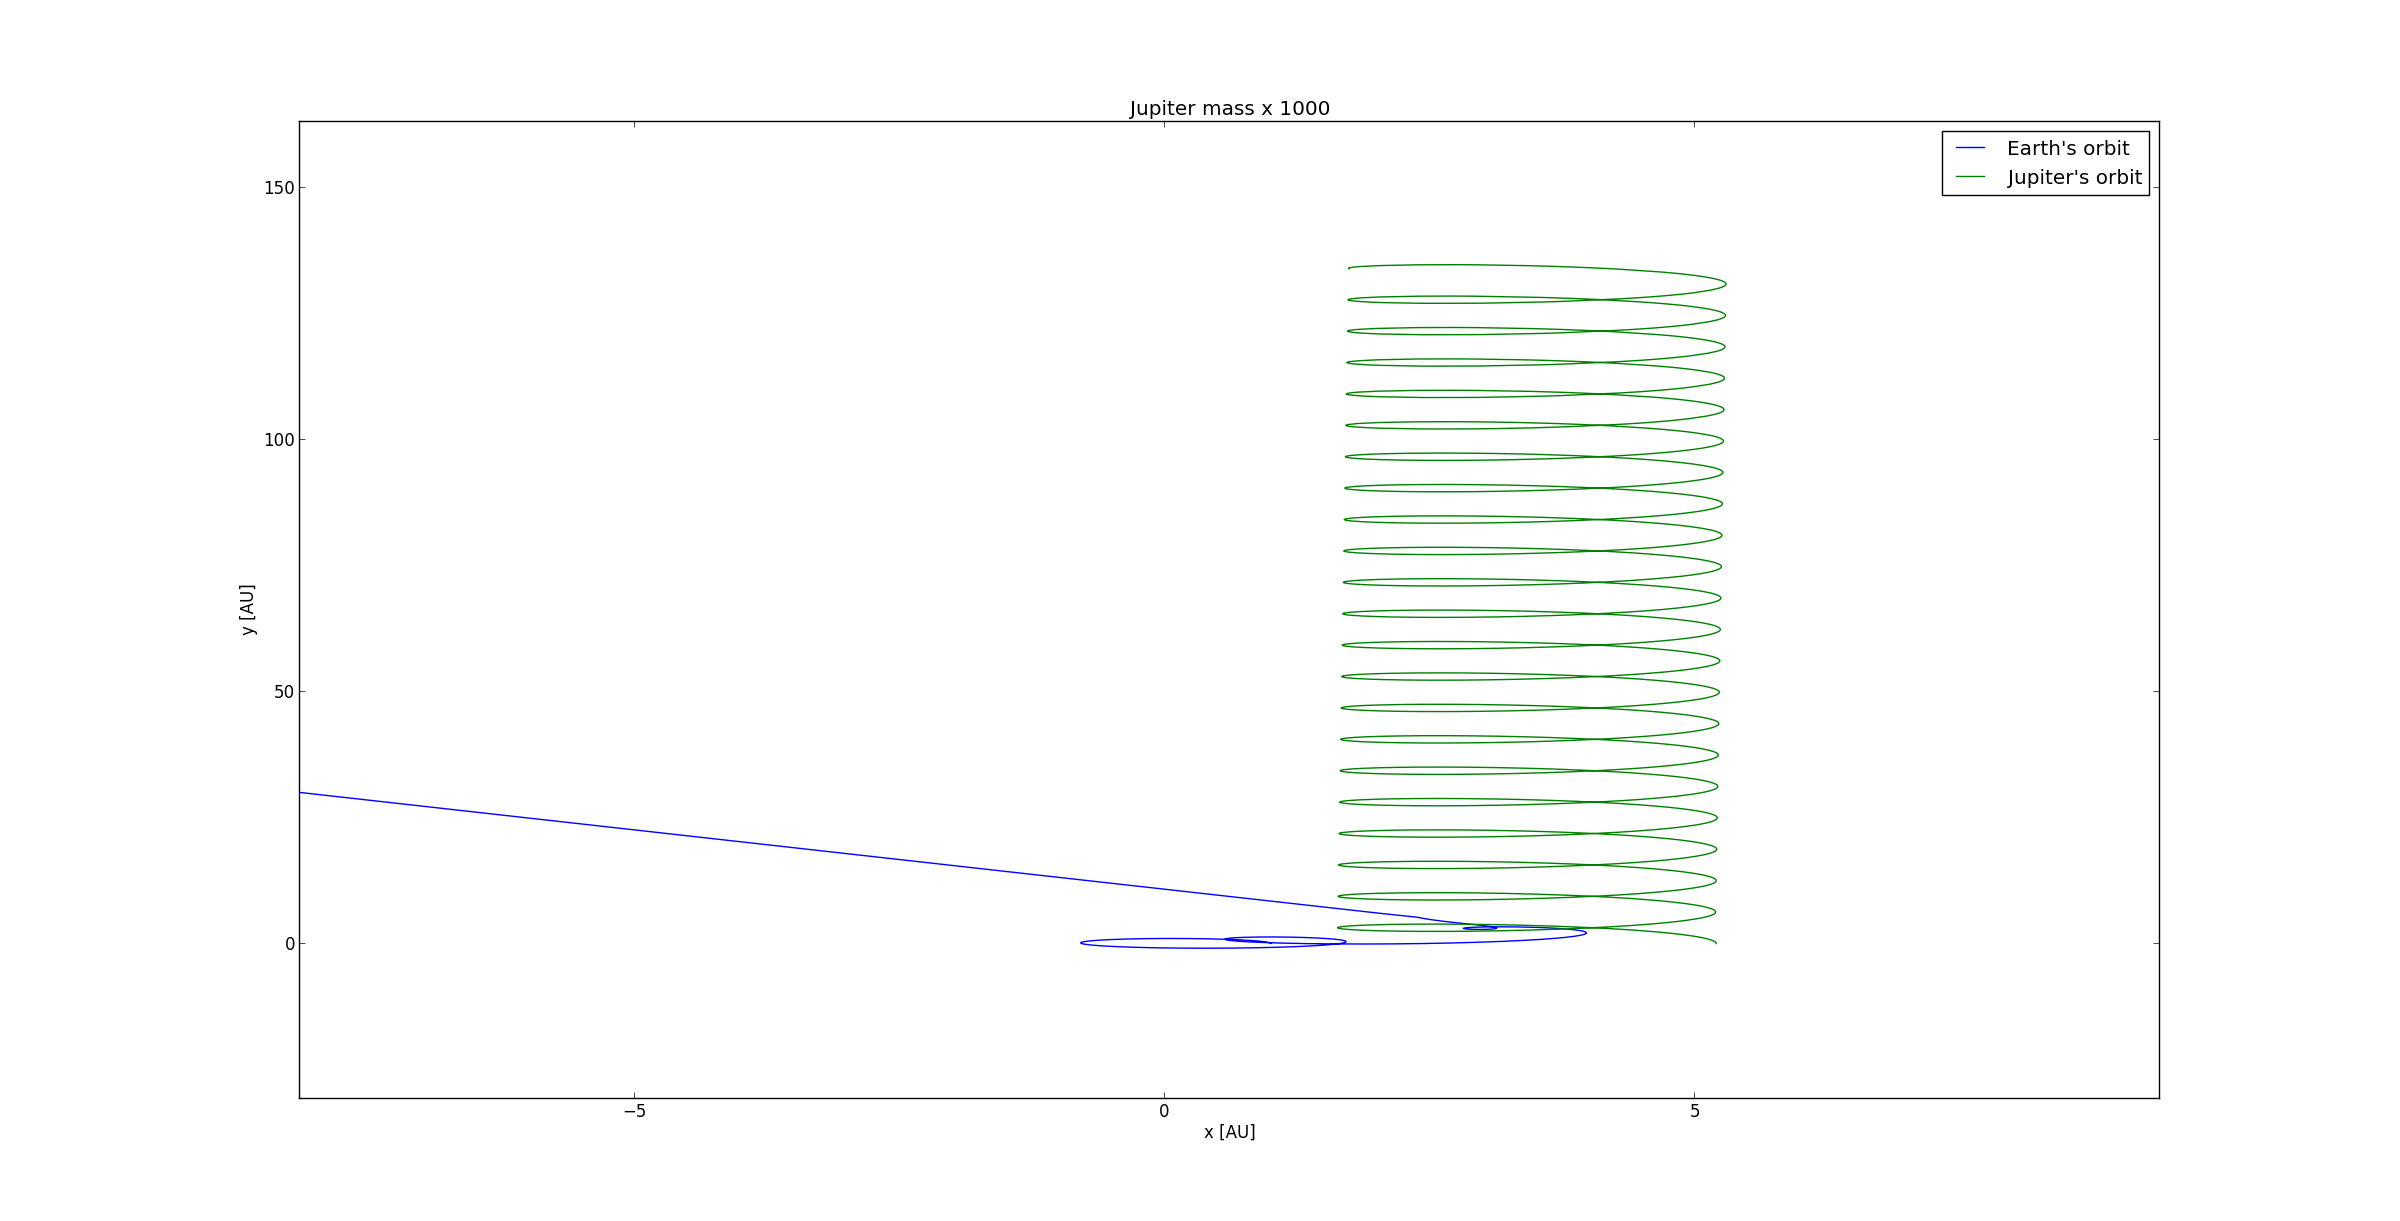
\includegraphics[scale=0.3]{figure_5.png}\\
We see that by increasing it by a factor of ten influences the earth's position far more vastly than what it had initially been. An increase by a factor of thousand results in something that odd and it could be a results of the failure of the algorithm, either way we see that Jupiter's mass influences the earth's position so vastly that it completely loses its orbit. The solution is no longer stable at this point and the results could not be used.   

Now giving the Sun an initial velocity in the $y$ and $x$ direction of $2$AU/yr on both directions gives us the following graph of the three planets in motion:\\
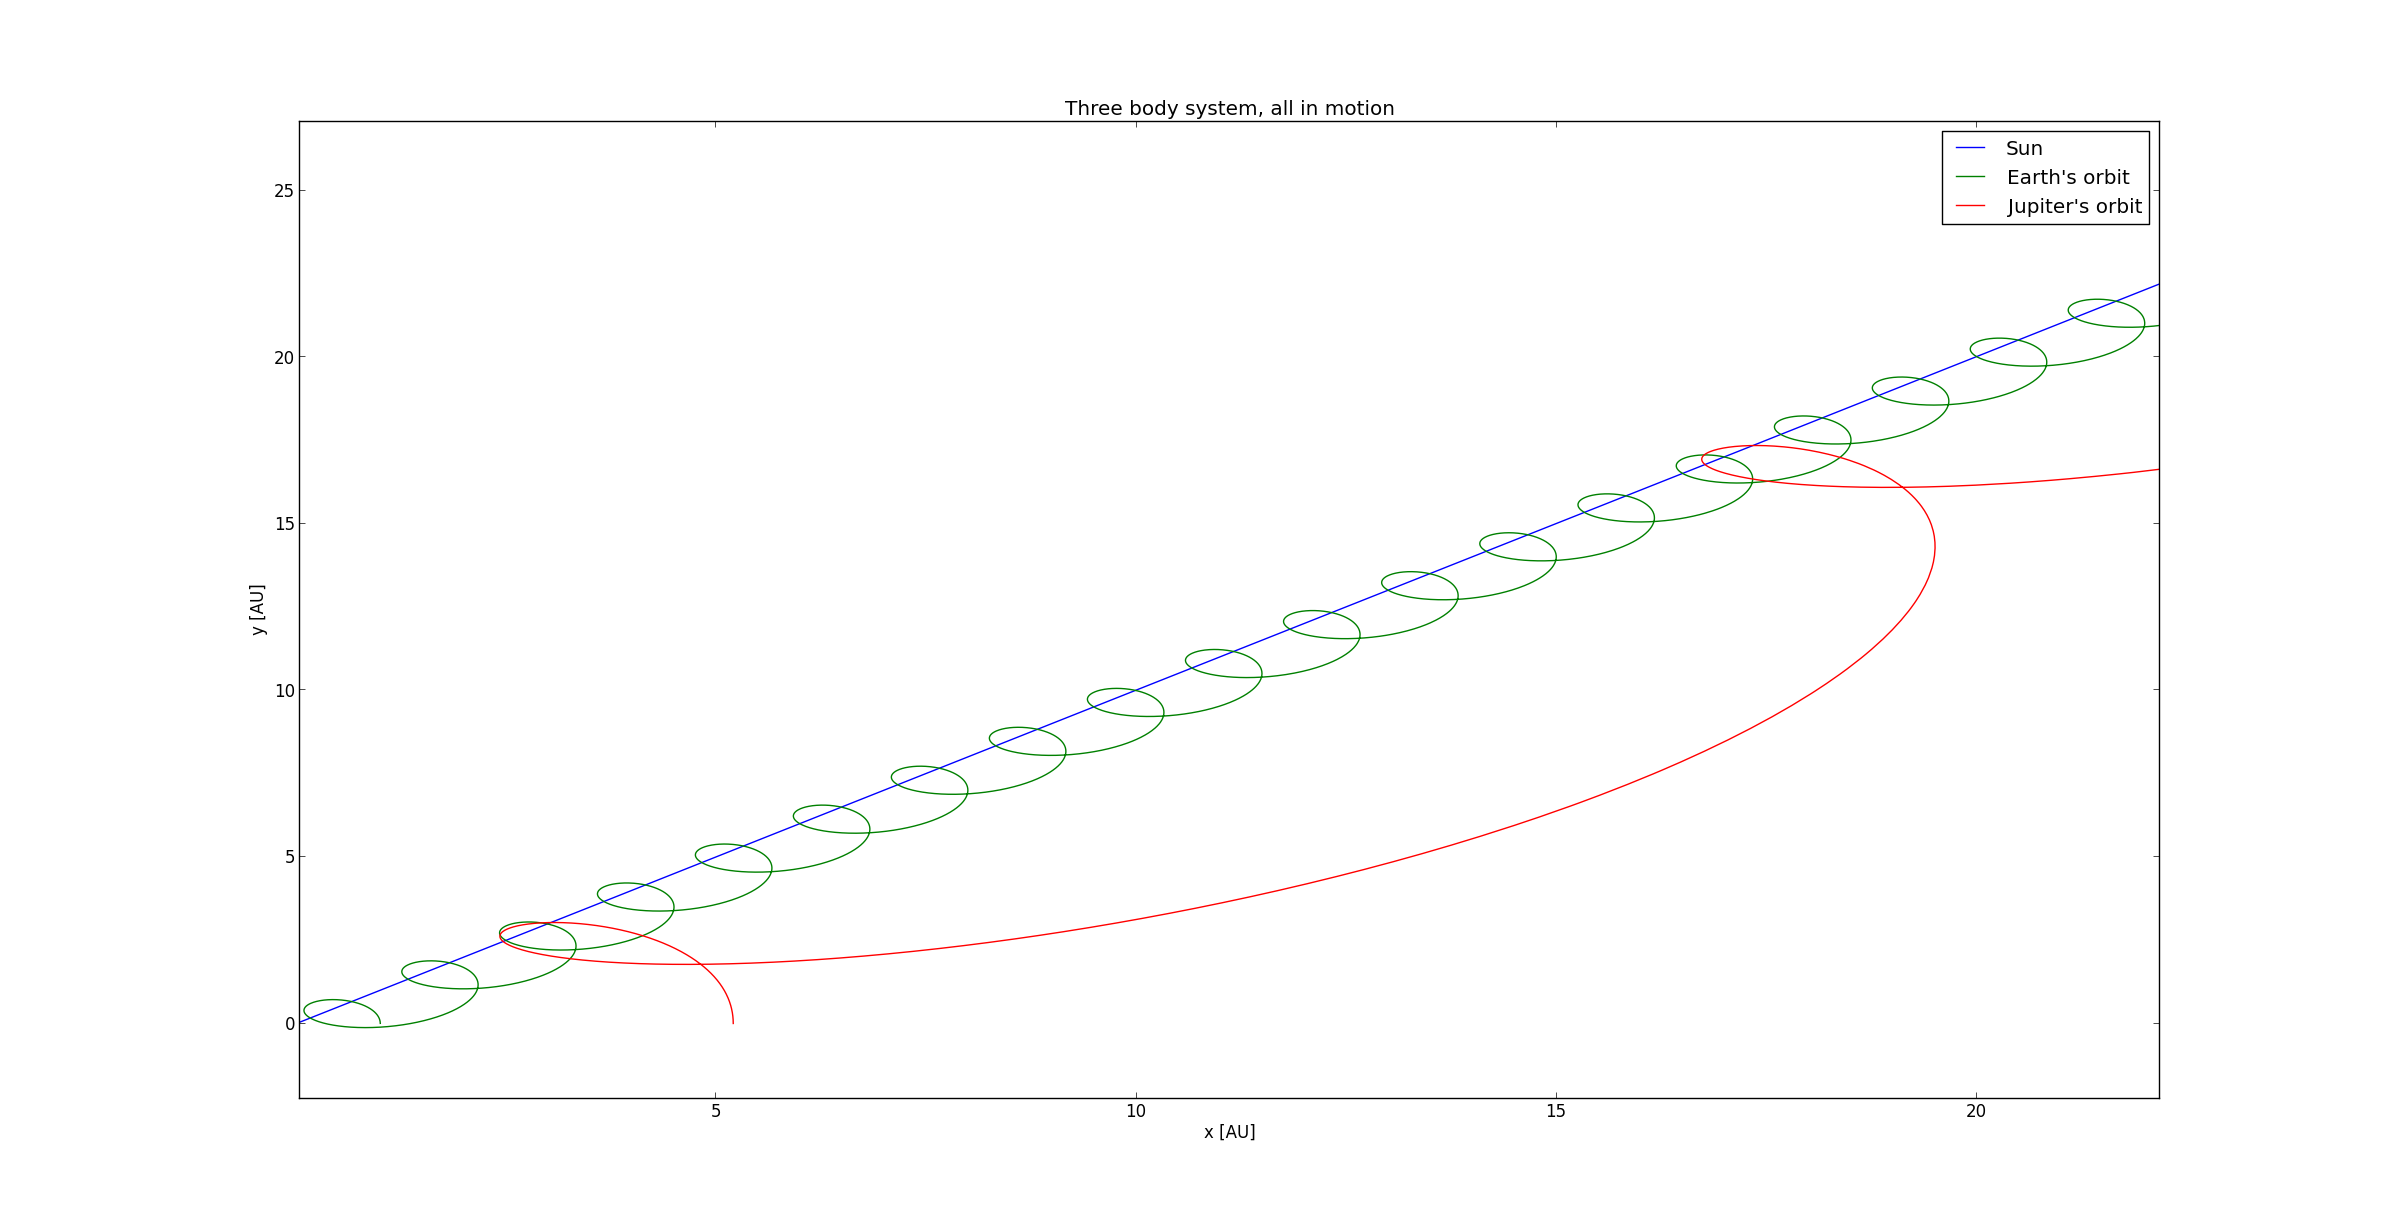
\includegraphics[scale=0.3]{figure_6.png}\\
From this we see that it takes longer for Jupiter to make one complete cycle compared to Earth, which is why I had to increase the number of iterations from around $1000~10000$ to $100000$ iterations. 

Now we include all planets with the Sun as our origin and we get:\\
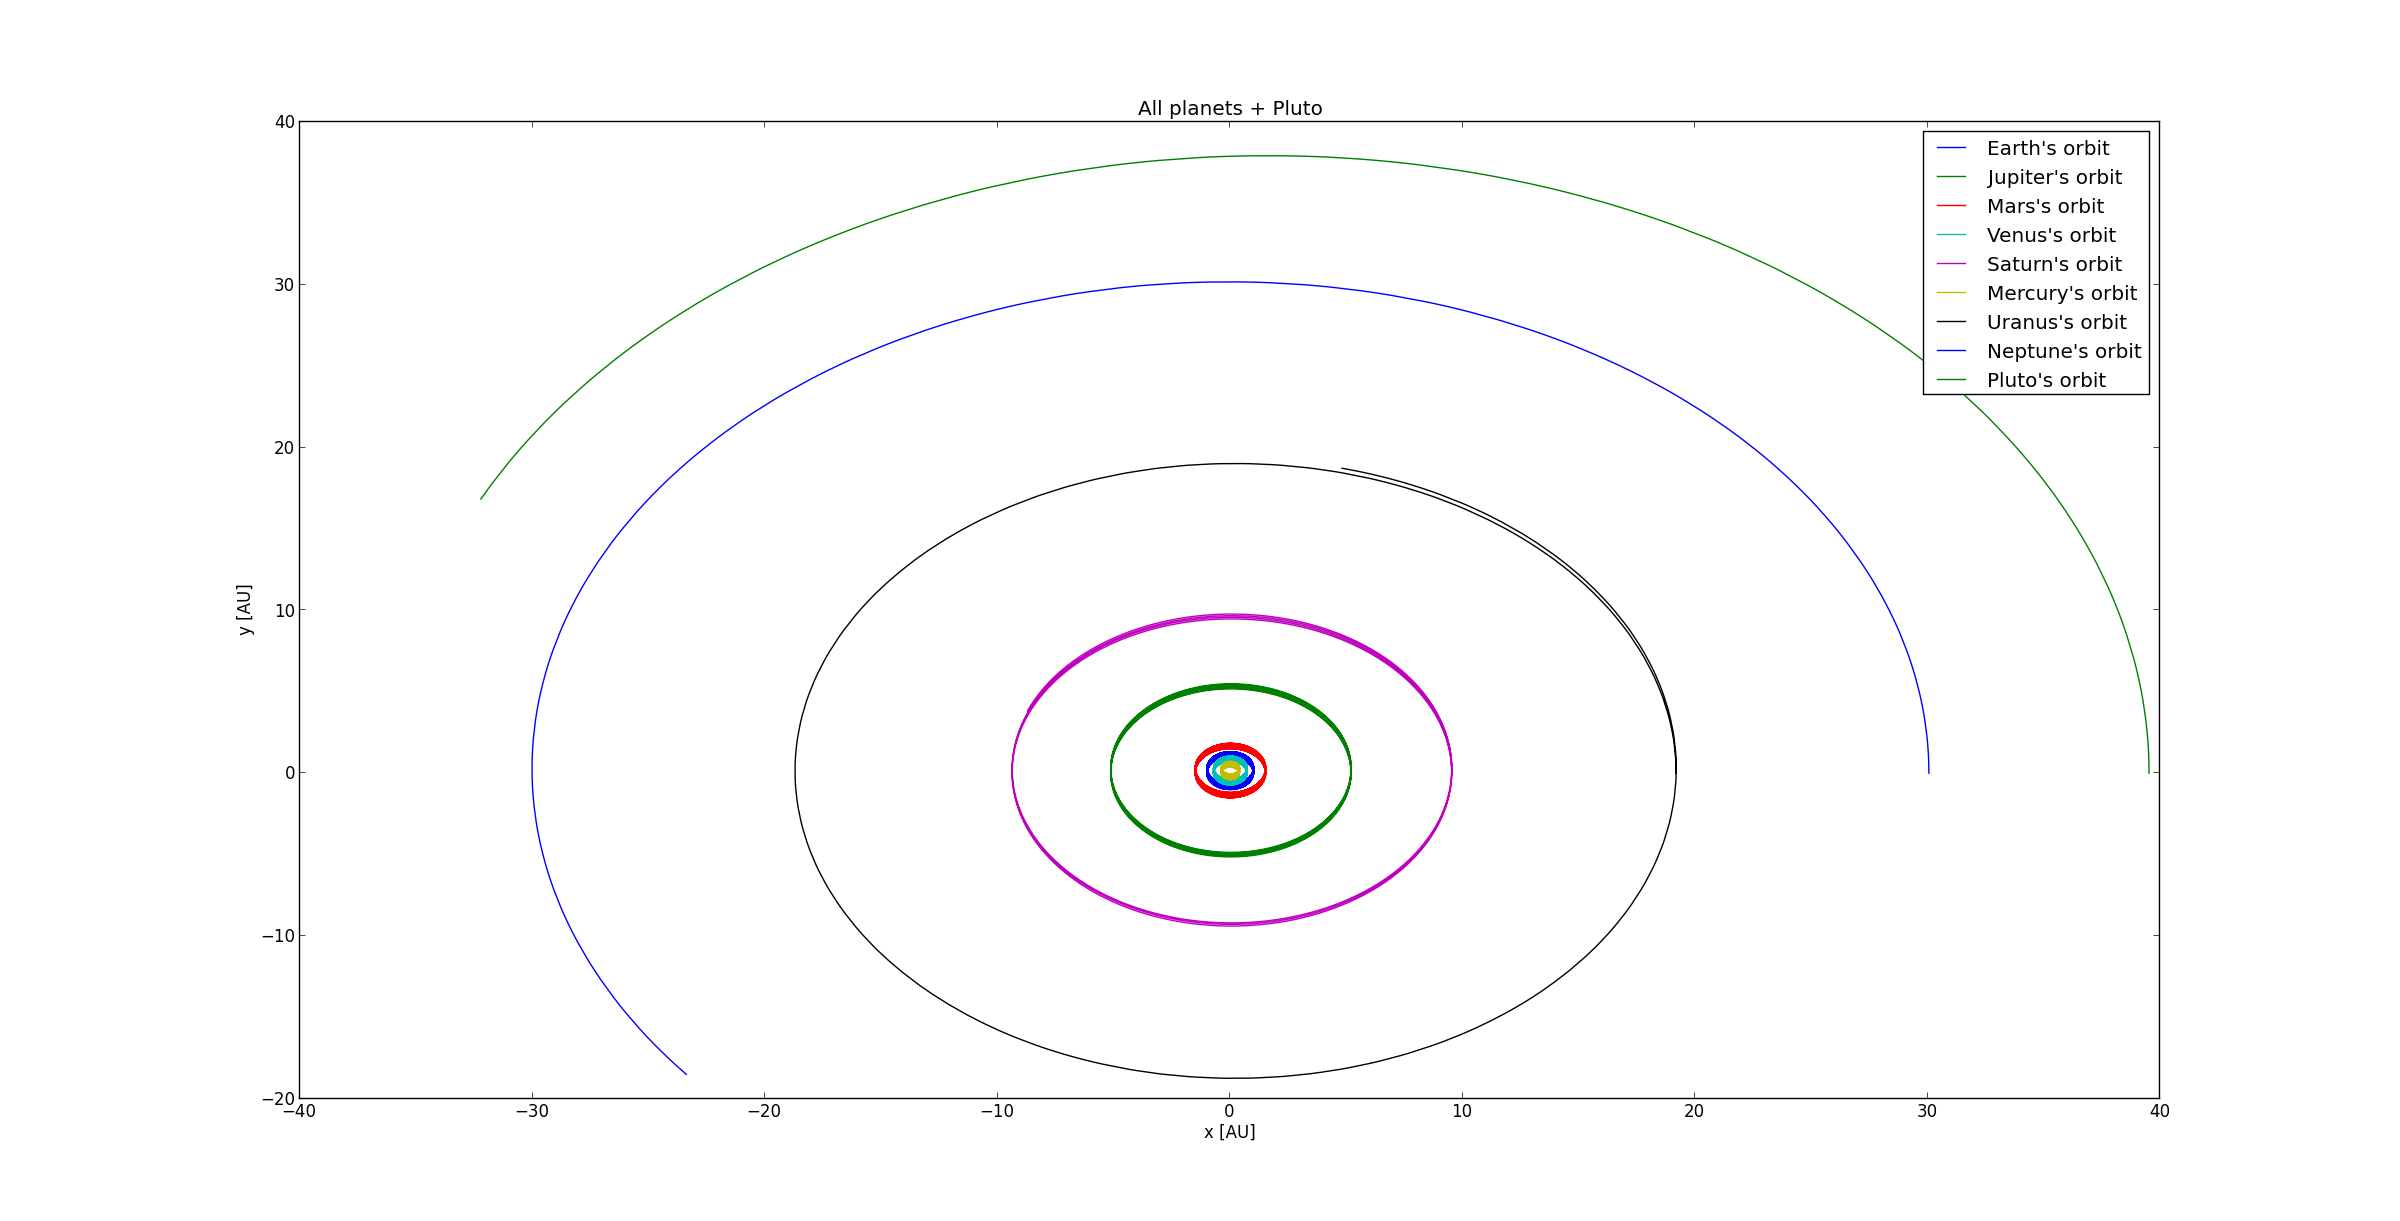
\includegraphics[scale=0.3]{figure_7.png}\\
As we can see the outer planets and Pluto take much longer to make a complete cycle and hence we have to increase our iteration time from $100000$ to $1000000$\\
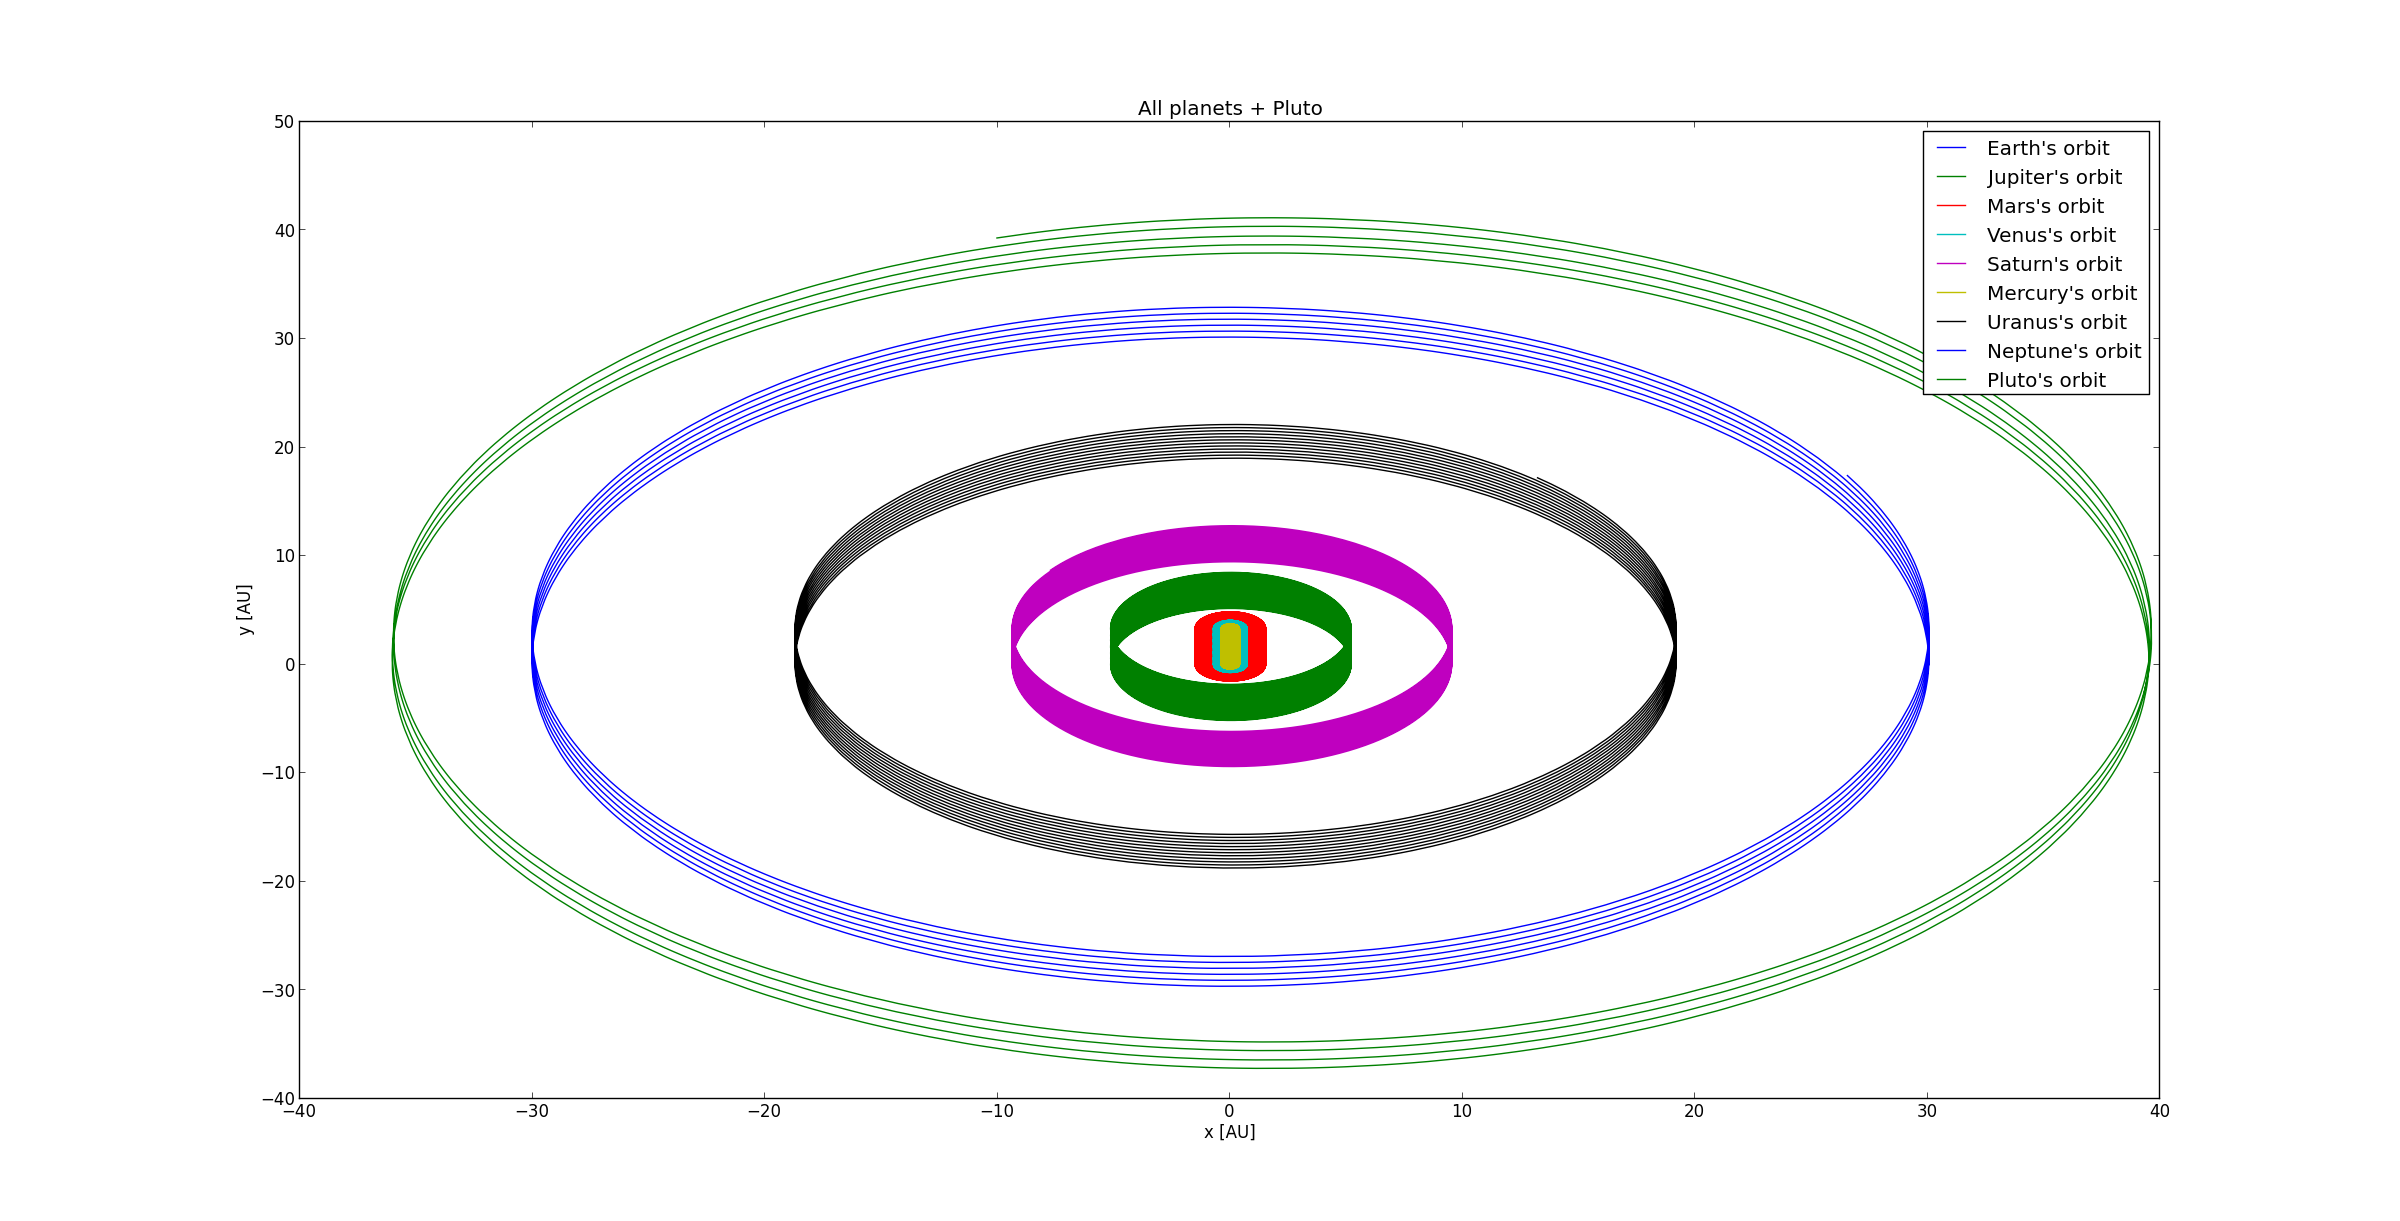
\includegraphics[scale=0.3]{figure_8.png}\\
But now we can no longer see clearly the orbits of the planets near the Sun for obvious reasons. 

\section{References}
https://github.com/Ace-/Project-3\\
Computational Physics, Morten Hjort-Jensen

\end{document}
 